
\de{ĐỀ THI HỌC KỲ II NĂM HỌC 2022-2023}{THPT Ngô Gia Tự - Đắk Lắk}
\begin{center}
	\textbf{PHẦN 1 - TRẮC NGHIỆM}
\end{center}
\Opensolutionfile{ans}[ans/ans]
\begin{ex}%[0D3Y1-1]%[Dự án đề kiểm tra HKII NH22-23- Võ Thị Thùy Trang]%[Ngô Gia Tự - ĐắkLắk]
	Biểu thức nào sau đây \textbf{không} là hàm số theo biến $x$?
	\choice
	{$y=5x^2-3x+4$}
	{$y=\sqrt{x^2-1}$}
	{$y=\left|2x+3\right|$}
	{\True $y^4=x^3$}
	\loigiai{
		Hàm số $y^4=x^3$ không phải là hàm số theo biến $x$ vì ứng với giá trị của $x=1$ có hai giá trị của $y$ là $y=1$ và $y=-1$.  	
	}
\end{ex}
\begin{ex}%[0D4Y2-1]%[Dự án đề kiểm tra HKII NH22-23- Võ Thị Thùy Trang]%[Ngô Gia Tự - ĐắkLắk]
	Tìm tập nghiệm $S$ của bất phương trình $x^2-4>0$.
	\choice
	{$S=\left(-\infty;-2\right]\cup \left[2;+\infty\right)$}
	{$S=\left(-\infty;0\right)\cup \left(4;+\infty\right)$}
	{$S=\left(-2;2\right)$}
	{\True $S=\left(-\infty;-2\right)\cup \left(2;+\infty\right)$}
	\loigiai{
		Ta có: $x^2-4>0 \Leftrightarrow  \left[\begin{aligned}
			&x<-2\\
			&x>2\\
		\end{aligned}\right.$. \\
		Vậy tập nghiệm của bất phương trình là $S=\left(-\infty;-2\right)\cup \left(2;+\infty\right)$.
	}
\end{ex}
\begin{ex}%[0X2Y2-1]%[Dự án đề kiểm tra HKII NH22-23- Võ Thị Thùy Trang]%[Ngô Gia Tự - ĐắkLắk]
	Có bao nhiêu cách xếp $4$ học sinh thành một hàng ngang?
	\choice
	{\True $4!$}
	{$4^2$}
	{$4^4$}
	{$4$}
	\loigiai{
		Số cách sắp xếp $4$ học sinh thành một hàng ngang là một hoán vị của $4$ phần tử. 	
	}
\end{ex}
\begin{ex}%[0X2B2-2]%[Dự án đề kiểm tra HKII NH22-23- Võ Thị Thùy Trang]%[Ngô Gia Tự - ĐắkLắk]
	Một tổ có $10$ công nhân. Có bao nhiêu cách chọn $2$ công nhân bất kỳ trong tổ làm $2$ chức vụ Nhóm trưởng và Nhóm phó?
	\choice
	{\True $90$}
	{$45$}
	{$100$}
	{$19$}
	\loigiai{
		Số cách chọn $2$ công nhân bất kỳ trong tổ làm $2$ chức vụ Nhóm trưởng và Nhóm phó là một chỉnh hợp chập $2$ của $10$ phần tử: $A_{10}^{2}=90$. 	
	}
\end{ex}
\begin{ex}%[0H4Y2-2]%[Dự án đề kiểm tra HKII NH22-23- Võ Thị Thùy Trang]%[Ngô Gia Tự - ĐắkLắk]
	Phương trình đường tròn $\left(C\right)$ có tâm $I\left(1;2\right)$ và bán kính $R=6$ là	
	\choice
	{$\left(x-1\right)^2+\left(y-2\right)^2=6$}
	{$\left(x+1\right)^2+\left(y+2\right)^2=6$}
	{$\left(x+1\right)^2+\left(y+2\right)^2=36$}
	{\True $\left(x-1\right)^2+\left(y-2\right)^2=36$}
	\loigiai{
		Phương trình đường tròn $\left(C\right)$ có tâm $I\left(1;2\right)$ và bán kính $R=6$ là $\left(x-1\right)^2+\left(y-2\right)^2=36$.	
	}
\end{ex}
\begin{ex}%[0H4B2-2]%[Dự án đề kiểm tra HKII NH22-23- Võ Thị Thùy Trang]%[Ngô Gia Tự - ĐắkLắk]
	Phương trình nào sau đây là phương trình của một đường tròn?
	\choice
	{$x^2+y^2-6x+4y+15=0$}
	{$3x^2+y^2-4x+2y-1=0$}
	{\True $x^2+y^2-4x+2y-1=0$}
	{$x^2+2y^2-2x+2y-1=0$}
	\loigiai{
		Phương trình đường tròn có dạng là: $x^2+y^2-2ax-2by+c=0$.\\
		Ta suy ra các phương trình $3x^2+y^2-4x+2y-1=0$ và $x^2+2y^2-2x+2y-1=0$ không phải là phương trình đường tròn.\\
		Xét phương trình $x^2+y^2-4x+2y-1=0$ ta có $a=2, b=-1, c=-1$.\\
		Khi đó: $a^2+b^2-c=2^2+(-1)^2-(-1)=6>0$ nên $x^2+y^2-4x+2y-1=0$ là phương trình đường tròn. 	
	}
\end{ex}
\begin{ex}%[0X2B2-2]%[Dự án đề kiểm tra HKII NH22-23- Võ Thị Thùy Trang]%[Ngô Gia Tự - ĐắkLắk]
	Số cách chọn $5$ học sinh trong một lớp có $25$ học sinh nam và $16$ học sinh nữ là
	\choice
	{\True $C_{41}^{5}$}
	{$A_{41}^{5}$}
	{$C_{25}^{5}+C_{16}^{5}$}
	{$C_{25}^{5}$}
	\loigiai{
		Tổng số học sinh của lớp là: $25+16=41$.\\
		Số cách chọn $5$ học sinh từ $41$ học sinh là một tổ hợp chập $5$ của $41$ phần tử: $C_{41}^{5}$. 	
	}
\end{ex}
\begin{ex}%[0D3Y1-3]%[Dự án đề kiểm tra HKII NH22-23- Võ Thị Thùy Trang]%[Ngô Gia Tự - ĐắkLắk]
	Cho hàm số $y=f(x)=2023x-2022$. Tính $f(1)$.
	\choice
	{$f(1)=2$}
	{$f(1)=2023$}
	{$f(1)=2022$}
	{\True $f(1)=1$}
	\loigiai{
		Ta có: $f(1)=2023 \cdot 1-2022=1$.	
	}
\end{ex}
\begin{ex}%[0X2B2-2]%[Dự án đề kiểm tra HKII NH22-23- Võ Thị Thùy Trang]%[Ngô Gia Tự - ĐắkLắk]
	Lớp 10A có $15$ học sinh nam và $25$ học sinh nữ. Có bao nhiêu cách chọn $1$ học sinh của lớp làm trực nhật?
	\choice
	{$15$}
	{\True $40$}
	{$25$}
	{$375$}
	\loigiai{
		Tổng số học sinh của lớp là: $15+25=40$.\\
		Số cách chọn $1$ học sinh của lớp làm trực nhật từ $40$ học sinh là một tổ hợp chập $1$ của $40$ phần tử: $C_{40}^{1}=40$. 	
	}
\end{ex}
\begin{ex}%[0D4Y3-2]%[Dự án đề kiểm tra HKII NH22-23- Võ Thị Thùy Trang]%[Ngô Gia Tự - ĐắkLắk]
	Số nào sau đây là nghiệm của phương trình $\sqrt{3x-2}+x=4$?
	\choice
	{$x=3$}
	{$x=1$}
	{\True $x=2$}
	{$x=0$}
	\loigiai{
		Ta có
		\allowdisplaybreaks
		\begin{eqnarray*}
		\sqrt{3x-2}+x=4  &\Rightarrow &\sqrt{3x-2}=4-x\\
		&  \Rightarrow & 3x-2=16-8x+x^2 \\
		& \Rightarrow & x^2-11x+18=0 \Rightarrow  \left[\begin{aligned}
			&x=9\\
			&x=2.\\
		\end{aligned}\right.	
		\end{eqnarray*}
		Thay lần lượt các giá trị trên vào phương trình đã cho ta thấy chỉ có $x=2$	thoả mãn.\\
		Vậy nghiệm của phương trình đã cho là $x=2$.
	}
\end{ex}
\begin{ex}%[0H4Y1-1]%[Dự án đề kiểm tra HKII NH22-23- Võ Thị Thùy Trang]%[Ngô Gia Tự - ĐắkLắk]
	Đường thẳng $\Delta\colon 2x+3y+2022=0$ có vectơ pháp tuyến có toạ độ là
	\choice
	{$\left(2022;2\right)$}
	{$\left(-3;2\right)$}
	{$\left(2;2022\right)$}
	{\True $\left(2;3\right)$}
	\loigiai{
		Đường thẳng $\Delta:2x+3y+2022=0$ có vectơ pháp tuyến là $\left(2;3\right)$.	
	}
\end{ex}
\begin{ex}%[0D4Y1-1]%[Dự án đề kiểm tra HKII NH22-23- Võ Thị Thùy Trang]%[Ngô Gia Tự - ĐắkLắk]
	Tìm khẳng định đúng trong các khẳng định sau
	\choice
	{$f(x)=2x-4$ là tam thức bậc hai}
	{\True $f(x)=3x^2+2x-5$ là tam thức bậc hai}
	{$f(x)=3x^3+2x-1$ là tam thức bậc hai}
	{$f(x)=x^4-x^2+1$ là tam thức bậc hai}
	\loigiai{
		Ta có: $f(x)=3x^2+2x-5$ là tam thức bậc hai	
	}
\end{ex}
\begin{ex}%[0X2B3-1]%[Dự án đề kiểm tra HKII NH22-23- Võ Thị Thùy Trang]%[Ngô Gia Tự - ĐắkLắk]
	Khai triển $\left(x-2\right)^4$ ta được 
	\choice
	{$\left(x-2\right)^4=x^4+8x^3-24x^2+32x-16$}
	{\True $\left(x-2\right)^4=x^4-8x^3+24x^2-32x+16$}
	{$\left(x-2\right)^4=x^4-8x^3-24x^2-32x-16$}
	{$\left(x-2\right)^4=x^4-16$}
	\loigiai{
		Ta có
		\allowdisplaybreaks
		\begin{eqnarray*}
			\left(x-2\right)^4&=&\mathrm{C}_{4}^{0}x^4+\mathrm{C}_{4}^{1}x^3(-2)+\mathrm{C}_{4}^{2}x^2(-2)^2+\mathrm{C}_{4}^{3}x(-2)^3+\mathrm{C}_{4}^{4}(-2)^4\\
			&=&x^4-8x^3+24x^2-32x+16.	
		\end{eqnarray*}	
	}
\end{ex}
\begin{ex}%[0D3Y2-1]%[Dự án đề kiểm tra HKII NH22-23- Võ Thị Thùy Trang]%[Ngô Gia Tự - ĐắkLắk]
	Hàm số nào sau đây không phải là hàm bậc hai?
	\choice
	{$f(x)=3+9x-2x^2$}
	{$f(x)=2.5x^2-2x$}
	{\True $f(x)=2022x+2023$}
	{$f(x)=x^2+1$}
	\loigiai{
		Hàm số $f(x)=2022x+2023$ là hàm số bậc nhất.	
	}
\end{ex}
\begin{ex}%[Dự án đề kiểm tra HKII NH22-23- Võ Thị Thùy Trang]%[Ngô Gia Tự - ĐắkLắk]
	Một hộp chứa $2$ bi vàng và $3$ bi đỏ. Lấy ngẫu nhiên $1$ viên bi từ hộp. Xác suất của biến cố $A\colon$\lq\lq Bi lấy ra có màu đỏ\rq\rq là
	\choice
	{$0{,}2$}
	{$0{,}4$}
	{\True $0{,}6$}
	{$0{,}3$}
	\loigiai{
		Không gian mẫu là $n(\Omega)=\mathrm{C}_{5}^{1}=5$.\\
		$n(A)=\mathrm{C}_{3}^{1}=3$.\\
		Xác suất của biến cố $A$ là\\
		$\mathrm{P}(A)=\dfrac{n(A)}{n(\Omega)}=\dfrac{3}{5}=0{,}6$. 	
	}
\end{ex}
\begin{ex}%[0H4B1-4]%[Dự án đề kiểm tra HKII NH22-23- Võ Thị Thùy Trang]%[Ngô Gia Tự - ĐắkLắk]
	Cho hai đường thẳng $d\colon 4x+3y-2022=0$ và $d'\colon 3x-4y+2023=0$. Góc giữa hai đường thẳng $d$ và $d'$ là
	\choice
	{$30^{\circ}$}
	{\True $90^{\circ}$}
	{$60^{\circ}$}
	{$45^{\circ}$}
	\loigiai{
		Đường thẳng $d$ có vectơ pháp tuyến là $\overrightarrow{n_{1}}=\left(4;3\right)$.\\ 
		Đường thẳng $d'$ có vectơ pháp tuyến là $\overrightarrow{n_{2}}=\left(3;-4\right)$.\\
		Ta có $\cos \left(d,d'\right)=\dfrac{4 \cdot 3+ 3 \cdot (-4)}{\sqrt{4^2+3^2} \cdot \sqrt{3^2+(-4)^2}}=0$.\\
		Vậy $\left(d,d'\right)=90^{\circ}$.	
	}
\end{ex}
\begin{ex}%[0X3B1-1]%[Dự án đề kiểm tra HKII NH22-23- Võ Thị Thùy Trang]%[Ngô Gia Tự - ĐắkLắk]
	Gieo một đồng xu liên tiếp hai lần. Số phần tử của không gian mẫu $n(\Omega)$ là
	\choice
	{$8$}
	{\True $4$}
	{$1$}
	{$2$}
	\loigiai{
		Gieo một đồng xu liên tiếp hai lần thì số phần tử của không gian mẫu là
		$n(\Omega)=2 \cdot 2=4$. 	
	}
\end{ex}
\begin{ex}%[0X2B1-2]%[Dự án đề kiểm tra HKII NH22-23- Võ Thị Thùy Trang]%[Ngô Gia Tự - ĐắkLắk]
	Một nhóm học sinh gồm $5$ bạn nam và $6$ bạn nữ. Có bao nhiêu cách chọn $2$ bạn từ nhóm gồm $1$ nam và $1$ nữ?
	\choice
	{$12$}
	{$55$}
	{\True $30$}
	{$11$}
	\loigiai{Có $5$ cách chọn bạn nam. Ứng với mỗi cách chọn bạn nam thì có $6$ cách chọn bạn nữ. Theo quy tắc nhân ta có $5\cdot6=30$ cách
	}
\end{ex}
\begin{ex}%[0X2Y2-8]%[Dự án đề kiểm tra HKII NH22-23- Võ Thị Thùy Trang]%[Ngô Gia Tự - ĐắkLắk]
	Số tổ hợp chập $2$ của $6$ bằng?
	\choice
	{\True $15$}
	{$6!$}
	{$12$}
	{$36$}
	\loigiai{Số tổ hợp chập $2$ của $6$ là $\mathrm{C}^2_6=15$
	}
\end{ex}
\begin{ex}%[0X2B2-8]%[Dự án đề kiểm tra HKII NH22-23- Võ Thị Thùy Trang]%[Ngô Gia Tự - ĐắkLắk]
	Có bao nhiêu số tự nhiên gồm $2$ chữ số khác nhau mà $2$ chữ số đều lẻ?
	\choice
	{\True $20$}
	{$40$}
	{$45$}
	{$50$}
	\loigiai{Số cách thành lập số tự nhiên gồm $2$ chứ số khác nhau mà $2$ chữ số đều lẻ là $\mathrm{A}^2_5=20$
	}
\end{ex}
\begin{ex}%[0X3B2-6]%[Dự án đề kiểm tra HKII NH22-23- Võ Thị Thùy Trang]%[Ngô Gia Tự - ĐắkLắk]
	Từ các chữ số $1,2,3,5,8,9$. Lấy ngẫu nhiên một số. Xác suất để lấy được số nguyên tố là
	\choice
	{\True $\dfrac{1}{2}$}
	{$\dfrac{1}{6}$}
	{$\dfrac{1}{4}$}
	{$\dfrac{1}{3}$}
	\loigiai{Gọi $\Omega$ là không gian mẫu. Ta có $n\left(\Omega\right)=6 $.\\ Gọi $A$ là biến cố lấy được số nguyên tố. Do đó $n\left( A\right)=3 $\\
		Xác suất cần tìm là $P\left(A \right)=\dfrac{n\left(A \right) }{n\left(\Omega \right)}=\dfrac{3}{6}=\dfrac{1}{2} $
	}
\end{ex}
\begin{ex}%[0H4Y2-1]%[Dự án đề kiểm tra HKII NH22-23- Võ Thị Thùy Trang]%[Ngô Gia Tự - ĐắkLắk]
	Cho đường tròng $\left(C\right)$ có phương trình$\colon\left(x-3\right)^2+\left(y+2\right)^2=25$. Toạ độ tâm $I$ và bán kính $R$ của đường tròn là?
	\choice
	{$I\left(2;-3\right)$ và $R=5$}
	{$I\left(-3;2\right)$ và $R=5$}
	{\True $I\left(3;-2\right)$ và $R=5$}
	{$I\left(3;-2\right)$ và $R=25$}
	\loigiai{Toạ độ tâm $I$ và bán kính $R$ của đường tròn là$\colon I\left(3;-2\right)$ và $R=5$
	}
\end{ex}
\begin{ex}%[0H4Y1-2]%[Dự án đề kiểm tra HKII NH22-23- Võ Thị Thùy Trang]%[Ngô Gia Tự - ĐắkLắk]
	Đường thẳng $d$ đi qua điểm $A\left(-2;-3\right)$ và có VTCP $\overrightarrow{u}=\left(-2;1\right)$ có phương trình là
	\choice
	{$\heva{&x=-2-2t\\&y=1-3t}$}
	{$\heva{&x=-2-3t\\&y=1-2t}$}
	{$\heva{&x=-2+t\\&y=-3-2t}$}
	{\True $\heva{&x=-2-2t\\&y=-3+t}$}
	\loigiai{Đường thẳng $d$ đi qua điểm $A\left(-2;-3\right)$ và có VTCP $\overrightarrow{u}=\left(-2;1\right)$ nên có phương trình là$\colon\heva{&x=-2-2t\\&y=-3+t}$
	}
\end{ex}
\begin{ex}%[0D3Y2-2]%[Dự án đề kiểm tra HKII NH22-23- Võ Thị Thùy Trang]%[Ngô Gia Tự - ĐắkLắk]
	\immini{
	Cho hàm số $y=f(x)=ax^2+bx+c$ có đồ thị như hình vẽ.
	Hàm số $f(x)<0$ với mọi $x$ thuộc khoảng?
	\choice
	{$\left(4;5\right)$}
	{$\left(-1;4\right)$}
	{$\left(0;1\right)$}
	{\True $\left(1;4\right)$}}
	{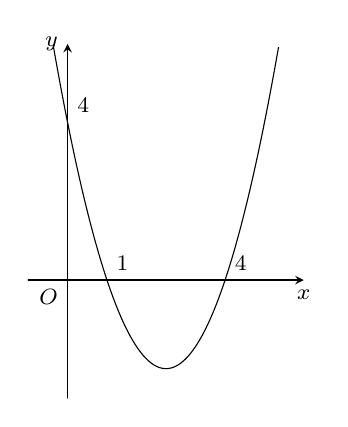
\begin{tikzpicture}[scale=.5,>=stealth, font=\footnotesize, line join=round, line cap=round]
			\def\a{1} \def\b{-5} \def\c{4} % Hệ số
			\def\xmin{-1} \def\xmax{6}
			\def\ymin{-3} \def\ymax{6}
			\draw[->] (\xmin,0)--(\xmax,0) node [below]{$x$};
			\draw[->] (0,\ymin)--(0,\ymax) node [left]{$y$};
			\node at (0,0) [below left]{$O$};
			\draw (1,0) node[above right] {$1$};
			\draw (4,0) node[above right] {$4$};
			\draw (0,4) node[above right] {$4$};
			\clip (\xmin+0.1,\ymin+0.1) rectangle (\xmax-0.5,\ymax-0.1);
			\draw[smooth,samples=300][domain=-1:6] plot(\x,{\a*(\x)^2+\b*(\x)+\c});
	\end{tikzpicture}}
	\loigiai{Dựa vào đồ thị ta có $f(x)<0\Leftrightarrow x\in\left(1;4\right)$ 
	}
\end{ex}
\begin{ex}%[0D3Y1-3]%[Dự án đề kiểm tra HKII NH22-23- Võ Thị Thùy Trang]%[Ngô Gia Tự - ĐắkLắk]
	Xét một phép thử có không gian mẫu $\Omega $ và $A$ là một biến cố của phép thử đó. Phát biểu nào sau đây \textbf{sai}?
	\choice
	{$0\le P\left(A\right)\le 1$}
	{Xác suất của biến cố $A$ là $P\left(A\right)=\dfrac{n\left(A\right)}{n\left(\Omega\right)}$}
	{$P\left(A\right)=1-P\left(\bar{A}\right)$}
	{\True $P\left(A\right)>1$}
	\loigiai{ Vì $0\le P\left(A\right)\le 1$ nên $P\left(A\right)>1$ là sai
	}
\end{ex}
\begin{ex}%[0H4Y3-2]%[Dự án đề kiểm tra HKII NH22-23- Võ Thị Thùy Trang]%[Ngô Gia Tự - ĐắkLắk]
	Trong các phương trình sau, phương trình nào là phương trình chính tắc của elip
	\choice
	{$x^2-y^2=1$}
	{$\dfrac{x^2}{64}+\dfrac{y^2}{16}=-1$}
	{\True $\dfrac{x^2}{9}+\dfrac{y^2}{4}=1$}
	{$\dfrac{x^2}{8}-\dfrac{y^2}{4}=1$}
	\loigiai{Phương trình chính tắc của elip là$\colon\dfrac{x^2}{9}+\dfrac{y^2}{4}=1$
	}
\end{ex}
\begin{ex}%[0H4B2-2]%[Dự án đề kiểm tra HKII NH22-23- Võ Thị Thùy Trang]%[Ngô Gia Tự - ĐắkLắk]
	Phương trình đường tròn $\left(C\right)$ có tâm $I\left(-1;2\right)$ và đi qua điểm $M\left(3;5\right)$ là?
	\choice
	{$\left(x+1\right)^2+\left(y-2\right)^2=5$}
	{\True $\left(x+1\right)^2+\left(y-2\right)^2=25$}
	{$\left(x-1\right)^2+\left(y+2\right)^2=25$}
	{$\left(x+1\right)^2+\left(y+2\right)^2=25$}
	\loigiai{Đường tròn $\left(C\right)$ có tâm $I\left(-1;2\right)$ và đi qua điểm $M\left(3;5\right)$ nên $R=IM=5$. Vậy phương trình đường tròn là$\colon\left(x+1\right)^2+\left(y-2\right)^2=25$
	}
\end{ex}
\begin{ex}%[0H4Y1-1]%[Dự án đề kiểm tra HKII NH22-23- Võ Thị Thùy Trang]%[Ngô Gia Tự - ĐắkLắk]
	Đường thẳng $\Delta\colon\heva{&x=1-t\\&y=3+2t}$. Véctơ chỉ phương có toạ độ là$\colon$
	\choice
	{$\left(-1;3\right)$}
	{\True $\left(-1;2\right)$}
	{$\left(-2;1\right)$}
	{$\left(1;3\right)$}
	\loigiai{ 	Đường thẳng $\Delta$ có phương trình $\colon\heva{&x=1-t\\&y=3+2t}$ nên véctơ chỉ phương có toạ độ là$\colon\vec{u}\left(-1;2\right)$
	}
\end{ex}
\begin{ex}%[0D2Y2-3]%[Dự án đề kiểm tra HKII NH22-23- Võ Thị Thùy Trang]%[Ngô Gia Tự - ĐắkLắk]
	Có bao nhiêu cách chọn $2$ viên bi bất kỳ từ một hộp đựng $5$ viên bi?
	\choice
	{$25$}
	{\True $10$}
	{$20$}
	{$15$}
	\loigiai{Số cách chọn $2$ viên bi bất kỳ từ một hộp đựng $5$ viên bi $C^2_5=10$
	}
\end{ex}
\begin{ex}%[0D3B2-6]%[Dự án đề kiểm tra HKII NH22-23- Võ Thị Thùy Trang]%[Ngô Gia Tự - ĐắkLắk]
	Cho tập hợp $S=\left\{2;3;4;5;6;7;8\right\}$. Chọn ngẫu nhiên một số từ tập hợp $S$, tính xác suất để số được chọn là số chẵn.
	\choice
	{$\dfrac{3}{8}$}
	{\True $\dfrac{4}{7}$}
	{$\dfrac{5}{7}$}
	{$\dfrac{3}{7}$}
	\loigiai{Ta có $n\left(S \right)=7$\\
		Gọi $A$ là biến cố "số được chọn là số chẵn"\\
		Do đó $n\left(A \right)=4 $\\
		Xác suất cần tìm là $P\left(A \right)=\dfrac{n\left(A \right) }{n\left(S \right) }=\dfrac{4}{7} $
	}
\end{ex}
\begin{ex}%[0H4Y3-8]%[Dự án đề kiểm tra HKII NH22-23- Võ Thị Thùy Trang]%[Ngô Gia Tự - ĐắkLắk]
	Phương trình nào sau đây là phương trình chính tắc của đường parabol?
	\choice
	{$x^2=-4y$}
	{$x^2=8y$}
	{$y^2=-8x$}
	{\True $y^2=80x$}
	\loigiai{ Phương trình chính tắc của đường parabol là $y^2=80x$ 
	}
\end{ex}
\begin{ex}%[0D4Y3-1]%[Dự án đề kiểm tra HKII NH22-23- Võ Thị Thùy Trang]%[Ngô Gia Tự - ĐắkLắk]
	Tập nghiệm của phương trình$\colon \sqrt{x^2+2x+3}=\sqrt{2x+4}$ là?
	\choice
	{$S=\left\lbrace 0;1\right\rbrace $}
	{$S=\left\lbrace -1;0\right\rbrace $}
	{\True $S=\left\lbrace -1;1\right\rbrace $}
	{$S=\left\lbrace 2;3\right\rbrace $}
	\loigiai{ Bình phương hai vế phương trình đã cho ta được$\colon$
		$$x^2+2x+3=2x+4\Leftrightarrow x^2-1=0\Leftrightarrow x=\pm 1$$
		Thử lại ta thấy $2$ nghiệm đều thoả mãn phương trình đã cho. 
	}
\end{ex}
\begin{ex}%[0X3B1-2]%[Dự án đề kiểm tra HKII NH22-23- Võ Thị Thùy Trang]%[Ngô Gia Tự - ĐắkLắk]
	Tung con súc sắc cân đối, đồng chất hai lần. Gọi $A$ là biến cố \lq\lq Số chấm xuất hiện cả hai lần giống nhau\rq\rq. Số kết quả thuận lợi của biến cố $A$ là
	\choice
	{$n(A)=36$}
	{$n(A)=12$}
	{\True $n(A)=6$}
	{$n(A)=2$}
	\loigiai{ Số kết quả thuận lợi của biến cố $A$ là$\colon n(A)=6$ 
	}
\end{ex}
\begin{ex}%[0H4B1-3]%[Dự án đề kiểm tra HKII NH22-23- Võ Thị Thùy Trang]%[Ngô Gia Tự - ĐắkLắk]
	Cho $2$ đường thẳng $d\colon x + y -2022=0$ và $d'\colon 2x - y + 2023=0$. Vị trí tương đối của hai đường thẳng là
	\choice
	{Vuông góc}
	{\True Cắt nhau}
	{Song song}
	{Trùng nhau}
	\loigiai{ Vì $\dfrac{1}{2}\ne \dfrac{1}{-1}$ nên hai đường thẳng $d$ và $d'$ cắt nhau
	}
\end{ex}
\begin{ex}%[0H4B1-5]%[Dự án đề kiểm tra HKII NH22-23- Võ Thị Thùy Trang]%[Ngô Gia Tự - ĐắkLắk]
	Trong mặt phẳng $Oxy$ cho điểm $M(1;1)$ và đường thẳng $d\colon 3x + 4y +8=0$. Khoảng cách từ $M$ đến
	đường thẳng $d$ là.
	\choice
	{$1$}
	{$4$}
	{\True $3$}
	{$2$}
	\loigiai{Ta có $d\left(M,d \right)=\dfrac{\left|3\cdot1+4\cdot1+8\right|}{\sqrt{3^2+4^2}}=3 $
	}
\end{ex}

\Closesolutionfile{ans}
\begin{center}
	\textbf{ĐÁP ÁN}
	\inputansbox{10}{ans/ans}	
\end{center}
\begin{center}
	\textbf{PHẦN 2 - TỰ LUẬN}
\end{center}

\begin{bt}%[0D8B3-1]%[Dự án đề kiểm tra HKII NH22-23- Võ Thị Thùy Trang]%[Ngô Gia Tự - ĐắkLắk]
Khai triển nhị thức $(2x+1)^4$.	
\loigiai{
	\allowdisplaybreaks
	\begin{eqnarray*}
		(2x+1)^4&=& \mathrm{C}_4^0(2x)^4+\mathrm{C}_4^1(2x)^3+\mathrm{C}_4^2(2x)^2+\mathrm{C}_4^3 2 x+\mathrm{C}_4^4\\
		&=& 16x^4+32x^3+24x^2+8x+1.
	\end{eqnarray*}
}
\end{bt}
\begin{bt}%[0D8B3-2]%[Dự án đề kiểm tra HKII NH22-23- Võ Thị Thùy Trang]%[Ngô Gia Tự - ĐắkLắk]
	Tìm số hạng chứa $x^2$ trong khai triển $(x+3)^5$.
	\loigiai{Số hạng cần tìm là $T_{k+1}=\mathrm{C}_5^kx^{5-k}\cdot 3^k$\\
	Theo bài ra $5-k=2$, vậy $k=3$ nên số hạng cần tìm là $10 \times 3^3\cdot x^2=270x^2$. }
\end{bt}
\begin{bt}%[0H9B2-2]%[Dự án đề kiểm tra HKII NH22-23- Võ Thị Thùy Trang]%[Ngô Gia Tự - ĐắkLắk]
	Trong mặt phẳng $(Oxy)$ cho điểm $M(2;4)$ và đường thẳng $d\colon 3x+y+2022=0$. Viết phương trình đường thẳng $d'$ song song với đường thẳng $d$ và cách điểm $M$ một khoảng bằng $\sqrt{10}$.
	\loigiai{
	Do $d'\parallel d$ nên $d'$ có phương trình dạng $3x+y+c=0$ với $c\ne 2022$.\\
	Ta có $\mathrm{d}(M,d')=\sqrt{10}$ nên $\dfrac{\left| 6+4+c\right|}{\sqrt{10}}=\sqrt{10}\Leftrightarrow\left| 10+c\right|=10$.\\
	Suy ra $10+c=10$ hoặc $10+c=-10$ hay $c=0$ hay $c=-20$.\\
	Vậy có $2$ đường thẳng thoã mãn ycbt là $d'\colon 3x+y=0$; $d'\colon 3x+y-20=0$.
	}
\end{bt}
\begin{bt}%[0T0K2-3]%[Dự án đề kiểm tra HKII NH22-23- Võ Thị Thùy Trang]%[Ngô Gia Tự - ĐắkLắk]
	Cho tập hợp $X=\{0,1,2,3,4,5,6,7\}$. Gọi $S$ là tập hợp tất cả các số tự nhiên có $5$ chữ số đôi một khác nhau được lập từ tập hợp $X$. Chọn ngẫu nhiên một số từ $S$. Tính xác suất để chọn được số chia hết cho $5$.
	\loigiai{
		Số tự nhiên có $5$ chữ số khác nhau $\overline{abcde}\quad (a\ne 0)$.\\
		Có $7$ cách chọn $a$.\\
		Có $7$ cách chọn $b$.\\
		Có $6$ cách chọn $c$.\\
		Có $5$ cách chọn $d$.\\
		Có $4$ cách chọn $e$.\\
		Vậy $n(\Omega)=7\cdot 7\cdot 6\cdot 5\cdot 4=5880$.\\
		Gọi $A$ là biến cố \lq\lq số được chọn chia hết cho $5$ \rq\rq.\\
		Khi đó $e=0$ hoặc $e=5$.\\
		với $e=0$.\\
		 Có $7$ cách chọn $a$.\\
		 Có $6$ cách chọn $b$.\\
		 Có $5$ cách chọn $c$.\\ 
		 Có $4 $cách chọn $d$.\\
		 với $e=5$.\\
		  Có $6$ cách chọn $a$.\\
		  Có $6$ cách chọn $b$.\\
		  Có $5$ cách chọn $c$.\\
		  Có $4$ cách chọn $d$.\\
		Vậy $n(A)=7\cdot 6\cdot 5\cdot 4+6\cdot 6\cdot 5\cdot 4=1560$.\\
		Xác suất của biến cố $A$ là  $\mathrm{P}(A)=\dfrac{1560}{5800}=\dfrac{13}{49}$.
	}
\end{bt}